% THIS DOCUMENT IS TAILORED TO REQUIREMENTS FOR SCIENTIFIC COMPUTING.  IT SHOULDN'T
% BE USED FOR NON-SCIENTIFIC COMPUTING PROJECTS
\documentclass[12pt]{article}

\usepackage{amsmath, mathtools}
\usepackage{amsfonts}
\usepackage{amssymb}
\usepackage{graphicx}
\usepackage{colortbl}
\usepackage{xr}
\usepackage{hyperref}
\usepackage{longtable}
\usepackage{xfrac}
\usepackage{tabularx}
\usepackage{float}
\usepackage{siunitx}
\usepackage{booktabs}
\usepackage{caption}
\usepackage{pdflscape}
\usepackage{afterpage}

\usepackage[round]{natbib}

%\usepackage{refcheck}

\hypersetup{
    bookmarks=true,         % show bookmarks bar?
      colorlinks=true,       % false: boxed links; true: colored links
    linkcolor=red,          % color of internal links (change box color with linkbordercolor)
    citecolor=green,        % color of links to bibliography
    filecolor=magenta,      % color of file links
    urlcolor=cyan           % color of external links
}



% For easy change of table widths
\newcommand{\colZwidth}{1.0\textwidth}
\newcommand{\colAwidth}{0.13\textwidth}
\newcommand{\colBwidth}{0.82\textwidth}
\newcommand{\colCwidth}{0.1\textwidth}
\newcommand{\colDwidth}{0.05\textwidth}
\newcommand{\colEwidth}{0.8\textwidth}
\newcommand{\colFwidth}{0.17\textwidth}
\newcommand{\colGwidth}{0.5\textwidth}
\newcommand{\colHwidth}{0.28\textwidth}

% Used so that cross-references have a meaningful prefix
\newcounter{defnum} %Definition Number
\newcommand{\dthedefnum}{GD\thedefnum}
\newcommand{\dref}[1]{GD\ref{#1}}
\newcounter{datadefnum} %Datadefinition Number
\newcommand{\ddthedatadefnum}{DD\thedatadefnum}
\newcommand{\ddref}[1]{DD\ref{#1}}
\newcounter{theorynum} %Theory Number
\newcommand{\tthetheorynum}{TM\thetheorynum}
\newcommand{\tref}[1]{TM\ref{#1}}
\newcounter{tablenum} %Table Number
\newcommand{\tbthetablenum}{TB\thetablenum}
\newcommand{\tbref}[1]{TB\ref{#1}}
\newcounter{assumpnum} %Assumption Number
\newcommand{\atheassumpnum}{A\theassumpnum}
\newcommand{\aref}[1]{A\ref{#1}}
\newcounter{goalnum} %Goal Number
\newcommand{\gthegoalnum}{GS\thegoalnum}
\newcommand{\gsref}[1]{GS\ref{#1}}
\newcounter{instnum} %Instance Number
\newcommand{\itheinstnum}{IM\theinstnum}
\newcommand{\iref}[1]{IM\ref{#1}}
\newcounter{reqnum} %Requirement Number
\newcommand{\rthereqnum}{R\thereqnum}
\newcommand{\rref}[1]{R\ref{#1}}
\newcounter{nfrnum} %NFR Number
\newcommand{\rthenfrnum}{NFR\thenfrnum}
\newcommand{\nfrref}[1]{NFR\ref{#1}}
\newcounter{lcnum} %Likely change number
\newcommand{\lthelcnum}{LC\thelcnum}
\newcommand{\lcref}[1]{LC\ref{#1}}

\usepackage{fullpage}

\newcommand{\deftheory}[9][Not Applicable]
{
\newpage
\noindent \rule{\textwidth}{0.5mm}

\paragraph{RefName: } \textbf{#2} \phantomsection 
\label{#2}

\paragraph{Label:} #3

\noindent \rule{\textwidth}{0.5mm}

\paragraph{Equation:}

#4

\paragraph{Description:}

#5

\paragraph{Notes:}

#6

\paragraph{Source:}

#7

\paragraph{Ref.\ By:}

#8

\paragraph{Preconditions for \hyperref[#2]{#2}:}
\label{#2_precond}

#9

\paragraph{Derivation for \hyperref[#2]{#2}:}
\label{#2_deriv}

#1

\noindent \rule{\textwidth}{0.5mm}

}

\begin{document}

\title{Software Requirements Specification for \progname: Guassian Mixture Model based on EM algorithm} 
\author{WONG, Kim Ying}
\date{\today}
	
\maketitle

~\newpage

\pagenumbering{roman}

\tableofcontents

~\newpage

\section*{Revision History}

\begin{tabularx}{\textwidth}{p{3cm}p{2cm}X}
\toprule {\bf Date} & {\bf Version} & {\bf Notes}\\
\midrule
1 Feb 2024 & 1.0 & SRS First Draft\\
\bottomrule
\end{tabularx}

~\\


~\newpage

\section{Reference Material}

This section records information for easy reference.

\subsection{Table of Units}

Throughout this document, we would consider all values to be unit-free. The rationale behind is that all units used in this document or model depend on the input dataset, while there is no general constraint on the unit of input. Therefore the input and the derived the statistical relation could be any units.
~\newline

\subsection{Table of Symbols}
\label{subsec:TOS}
The table that follows summarizes the symbols used in this document along with
their units (if exists). The choice of symbols was made to be consistent with the statistics literature and with existing documentation for the Gaussian Mixture Model. The symbols are listed in alphabetical order.

\renewcommand{\arraystretch}{1.2}
%\noindent \begin{tabularx}{1.0\textwidth}{l l X}
\noindent \begin{longtable*}{l l p{12cm}} \toprule
\textbf{symbol} & \textbf{Description}\\
\midrule 
            M         & number of data-points  \\
                        N         &number of predictor variables \\
                                    K        & number of clusters needed  \\
                                                z & latent variable in GMM\\

                                                        p(x) & Gaussian mixture distribution\\
$\Sigma$ &    covariance  \\
$\mu$ &    mean           \\
$\pi$ &    mixing coefficient   \\
            $N(\mu_{k} , \Sigma_{k} ) $ & Gaussian distribution with mean $\mu$ and variance $\Sigma$\\
                        p(x) & probability density function \\
                         \gamma(z_{k})  & responsibility
            
\\ 
\bottomrule
\end{longtable*}


\subsection{Abbreviations and Acronyms}

\renewcommand{\arraystretch}{1.2}
\begin{tabular}{l l} 
  \toprule		
  \textbf{symbol} & \textbf{description}\\
  \midrule 
  A & Assumption\\
  DD & Data Definition\\
  GD & General Definition\\
  GS & Goal Statement\\
  IM & Instance Model\\
  LC & Likely Change\\
  PS & Physical System Description\\
  R & Requirement\\
  SRS & Software Requirements Specification\\
  \progname{} & \plt{put an expanded version of your program name here (as appropriate)}\\
  TM & Theoretical Model\\
  GMM & Gaussian Mixture Model\\
  EM & Expectation Maximization \\
  GMM-EM & Software Name \\
  \bottomrule
\end{tabular}\\

\plt{Add any other abbreviations or acronyms that you add}

\subsection{Mathematical Notation}

\plt{We borrow the convention for mathematical notation from the book Pattern Recognition and Machine Learning. \\
Typographic Conventions: \\
We denote vector as a lowercase bold roman letters such as \textbf{x}. Matrices are denoted by uppercase bold roman letters such as \textbf{M}. A single real-valued variable will be denoted as a lowercase roman letter such as x. \\
We introduce the notation for conditional probability as: $p(Y|X)$ as the probability of Y given X, where X is the marginal probability, or simply called probability of X; and the joint probability is defined as: $p(X,Y)$. The normal distribution with mean $\mu$ and  covariance $\Sigma$ is denoted as $N(\mu, \Sigma)$. These notation could be generalized to higher dimension by replacing real-valued numbers with vectors or matrices.  }

\newpage

\pagenumbering{arabic}

\section{Introduction}

\plt{Mixture model is a probabilistic model that describes the datasets or measurement in a linear combination of some basic distributions. Gaussian mixture model falls into a subset of the mixture model, where Gaussian distribution is used as a basis. In general, almost all continuous density could be approximated as sufficient number of Gaussian mixtures with appropriate mean and covariance. \\
Therefore, it can be used in various cases in machine learning, such as clustering and density estimation. The GMM-EM aims at implementation of the Gaussian mixture model for clustering fundamentally. This section is divided into 4 parts: }

\begin{itemize}

\item \ref{subsec:pod} Purpose of document 
\item \ref{subsec:sor} Scope of requirements
\item \ref{subsec:cir} Characteristics of Intended reader 
\item \ref{subsec:ood} Organization of document
\end{itemize}

\subsection{Purpose of Document} 
\label{subsec:pod}

\plt{The document serves as a outline for the requirement specification for the GMM-EM. The reader could refer to this document for the general and specific system description. Theoretical model and their assumption will be detailed in this document.}

\subsection{Scope of Requirements} 
\label{subsec:sor}
\plt{The GMM-EM would be a general library in implementation of Gaussian mixture model based on the EM algorithm with a fundamental focus in clustering problem. We will limit to deal with any dataset with only real-valued number without any missing value. The software would  guarantee a convergence in solution but not the optimality. }  

\subsection{Characteristics of Intended Reader} \label{sec_IntendedReader}
\label{subsec:cir}
\plt{The intended readers should acquire basic understanding on linear algebra, calculus and statistics, preferably exposure on the basic statistical learning algorithm. Undergraduate introduction courses in these topics should suffix the above requirements.}

\subsection{Organization of Document}
\label{subsec:ood}
\plt{The document consist of 5 parts: }

\begin{itemize}

\item Section \ref{sec:gsd} General System Description
\item Section \ref{sec:ssd} Specific System Description
\item Section \ref{sec:req} Requirements
\item Section \ref{sec:lc} Likely Changes and Section \ref{sec:uc} Unlikely Changes
\item Section \ref{sec:tmg} Traceability Matrices and Graphs
\end{itemize}

\section{General System Description}
\label{sec:gsd}
This section provides general information about the software GMM-EM. It consists of three parts:
\begin{itemize}
    \item \ref{subsec:sct} System Context
    \item \ref{subsec:uc}  User Characteristics
\end{itemize}

\subsection{System Context}
\label{subsec:sct}
\plt{The software follows the structure as Figure shown. The user is supposed to input a real-valued dataset as a matrix to the GMM-EM. The GMM-EM will give an array which contains the predicted label for each data points in the dataset. }
\begin{figure}[h!]
\begin{center}
 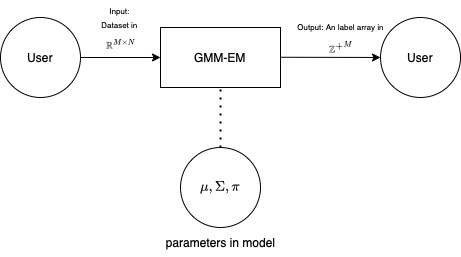
\includegraphics[width=0.6\textwidth]{system_context.jpg}
\caption{System Context}
\label{Fig_SystemContext} 
\end{center}
\end{figure}



\begin{itemize}
\item User Responsibilities:
\begin{itemize}
\item Provides a real-valued number of dataset without missing value in a matrix form
\item Specify the number of clusters needed (optional)
\end{itemize}
\item \progname{} GMM-EM Responsibilities:
\begin{itemize}
\item Detect any wrong data type in input like containing string
\item Return an array of label for each data point to which cluster it should belong. 
\item Identify the number of clusters needed if users do not provide 
\end{itemize}
\end{itemize}

\subsection{User Characteristics} \label{SecUserCharacteristics}
\label{subsec:uc}
\plt{The user should acquire basic programming skill and be able to perform data preprocessing for a dataset. It is also preferable that users know some common libraries in handling different data formats such as csv or json.}

\section{Specific System Description}
\label{sec:ssd}

\begin{itemize}

\item Section \ref{subsec_pd} Problem Description
\item Section \ref{subsec:scs} Solution Characteristics Specification

\end{itemize}

This section first presents the problem description, which gives a high-level
view of the problem to be solved.  This is followed by the solution characteristics
specification, which presents the assumptions, theories, definitions and finally
the instance models. 

\subsection{Problem Description} 
\label{subsec_pd}

\progname{GMM-EM} is intended to implement a library on Gaussian Mixture model which is specifically used in clustering. 
\plt{The software tackle a 
general clustering problem for different datasets }

\subsubsection{Terminology and Definitions}

\plt{In this section, we would explain the terminology used in our theoretical model. }

\begin{itemize}

\item Likelihood function: The degree of similarity of the observed dataset similar to                            what we guess about the data points
\item mixture of Gaussian: data points where are from different                                                   Gaussian distributions
\end{itemize}


\subsubsection{Goal Statements}

\noindent Given the \plt{a dataset without missing value and infinity value which perferably designed for clustering or classification }, the goal statements are:

\begin{itemize}

\item[GS\refstepcounter{goalnum}\thegoalnum \label{G_meaningfulLabel}:] \plt{Predict which cluster should each data point belongs to}

\item[GS\refstepcounter{goalnum}\thegoalnum \label{G_meaningfulLabel}:] \plt{Detect how many clusters should use if number of cluster are not specified}


\end{itemize}

\subsection{Solution Characteristics Specification}
\label{subsec:scs}
\plt{This section illustrate the theory which \progname{GMM-EM fundamentally relied on. We start from statistical assumption, to statistical theorem and definitions and the provide more details on the mathematical foundation about the training process for \progname{GMM-EM} }}
The instance models that govern \progname{} are presented in
Subsection~\ref{sec_instance}.  The information to understand the meaning of the
instance models and their derivation is also presented, so that the instance
models can be verified.


\subsection{Scope Decisions}

\plt{The \progname{GMM-EM} will fundamentally focus on the real-valued dataset which is designed for clustering or classification. Other GMM features or application such as density estimation may not be provided in our library.}


\subsubsection{Assumptions} \label{sec_assumpt}

\begin{itemize}

\item[A\refstepcounter{assumpnum}\theassumpnum \label{A_meaningfulLabel}:]
  \plt{We assume properties of probability density function holds here, which include non-negativity and normalization}
 
\item[A\refstepcounter{assumpnum}\theassumpnum \label{A_meaningfulLabel}:]
  \plt{We assume the dataset could be approximated by mixtures of Gaussian.}

\item[A\refstepcounter{assumpnum}\theassumpnum \label{A_meaningfulLabel}:]
  \plt{We assume the dataset is real-valued without any missing value.}
  
  
\end{itemize}

\subsubsection{Theoretical Models}\label{sec_theoretical}

\plt{In this section, we will introduce the theoretical foundation for the \progname{GMM-EM}. It fundamentally relied on the fact the data could always approximated by a mixture of Gaussian. The mathematical formulation is listed below.}

~\newline

\noindent
\deftheory
% #2 refname of theory
{TM:GMM}
% #3 label
{mixture of Gaussian }
% #4 equation
{
  $p(\textbf{x}) = \sum_{k=1}^{K}  \pi_{k} N(x | \mathbf{\mu_{k}} , \mathbf{\Sigma_{k}} )$ with 
  $ 0 \leq \pi_{k} \leq 1 $ and $\sum_{k=1}^{K}\pi_{k} = 1 $
}
% #5 description
{
  The above equation gives the mathematical formulation on GMM. It states that for a Gaussian mixture distribution, it could be written as the linear combination of Gaussian distribution with a certain covariance  {$\mathbf{\Sigma_{k}}$} and mean $\mathbf{\mu_{k}}$. From the normalization and non-negativity of the probability density function, the condition for mixing coefficient is imposed as above. It is a direct result from our basic assumption (A1). 
}
% #6 Notes
{
None.
}
% #7 Source
{
  Pattern Recognition and Machine Learning by Christopher M. Bishop
}
% #8 Referenced by
{
  \dref{LLF},  \dref{Res}
}
% #9 Preconditions
{
None
}
% #1 derivation - not applicable by default
{}

~\newline

\deftheory
% #2 refname of theory
{TM:BT}
% #3 label
{Bayes' Theorem }
% #4 equation
{
  $P(Y | X) = \frac{P(X | Y) \cdot P(Y)}{P(X)}$ 
}
% #5 description
{
  The above equation gives the mathematical foundation on Bayesian Statistics. This define the Log likelihood function which will be maximized in parameter training process. 
}
% #6 Notes
{
None.
}
% #7 Source
{
  Pattern Recognition and Machine Learning by Christopher M. Bishop
}
% #8 Referenced by
{
  \dref{LLF}, \dref{Res}
}
% #9 Preconditions
{
None
}
% #1 derivation - not applicable by default
{}

~\newline

\subsubsection{General Definitions}\label{sec_gendef}

\plt{We will define the Log Likelihood function and responsibilities in this section. The maximization in Log likelihood function will be key for training the \progname{GMM-EM}. }

\\
~\newline

\noindent
\begin{minipage}{\textwidth}
\renewcommand*{\arraystretch}{1.5}
\begin{tabular}{| p{\colAwidth} | p{\colBwidth}|}
\hline
\rowcolor[gray]{0.9}
Number& GD\refstepcounter{defnum}\thedefnum \label{Res}\\
\hline
Label &\bf Responsibility \\
\hline
% Units&$MLt^{-3}T^0$\\
% \hline

Equation&$ \gamma(z_{k}) = \frac{\pi_{k} N(\mathbf{x} | \mathbf{\mu_{k}} ,\mathbf{\Sigma_{k}} )}{\sum_{j=1}^{K}  \pi_{k} N(\mathbf{x} | \mathbf{\mu_{j}} ,\mathbf{\Sigma_{j}} )}$  \\
\hline
Description &
The responsibility is defined as conditional probability of a latent variable \textbf{z} given that we know about \textbf{x}. We could under this as given that a data point, how probable it would be in a certain cluster (which could be interpreted as one-hot encoding of \textbf{z} ) The mathematical symbols are defined in Section \ref{subsec:TOS}
\\
\hline
  Source & Pattern Recognition and Machine Learning by Christopher M. Bishop \\
  \hline
  Ref.\ By & \iref{EM} \\
  \hline
\end{tabular}
\end{minipage}
\\
~\newline
\noindent
\begin{minipage}{\textwidth}
\renewcommand*{\arraystretch}{1.5}
\begin{tabular}{| p{\colAwidth} | p{\colBwidth}|}
\hline
\rowcolor[gray]{0.9}
Number& GD\refstepcounter{defnum}\thedefnum \label{LLF}\\
\hline
Label &\bf Log likelihood function \\
\hline
% Units&$MLt^{-3}T^0$\\
% \hline

Equation&$    \ln p(\mathbf{X} | \mathbf{\pi} , \mathbf{\mu} ,\mathbf{ \Sigma}) = \sum_{n=1}^{N} ln {\sum_{k=1}^{K}  \pi_{k} N(\mathbf{x} | \mathbf{\mu_{k}} ,\mathbf{\Sigma_{k}} )$  \\
\hline
Description &
Likelihood function is a direct result from given by the expression of Gaussian mixture with the Bayes' Theorem. We impose the log scale to the likelihood and obtain the log likelihood function. The mathematical symbols are defined in Section \ref{subsec:TOS}
\\
\hline
  Source & Pattern Recognition and Machine Learning by Christopher M. Bishop \\
  \hline
  Ref.\ By &  \iref{EM} \\
  \hline
\end{tabular}
\end{minipage}\\

\subsubsection{Instance Models}   

\plt{We will outline the EM part in GMM-EM. Instead of giving details in implementation, we will provide a rather abstract but mathematically non-rigorous treatment in this section. } 

~\newline

%Instance Model 1

\noindent
\begin{minipage}{\textwidth}
\renewcommand*{\arraystretch}{1.5}
\begin{tabular}{| p{\colAwidth} | p{\colBwidth}|}
  \hline
  \rowcolor[gray]{0.9}
  Number& IM\refstepcounter{instnum}\theinstnum \label{EM}\\
  \hline
  Label& \bf EM Algorithm \\
  \hline
  Input& Initialized $\mathbf{\pi_{k}}  , \mathbf{\mu_{k}} ,\mathbf{\Sigma_{k}} $ based on the input dataset \textbf{X} $\in \mathbb{R}^{M\times N}$  \\
  \hline
  Output& Best parameter in $\mathbf{\pi_{k}}  , \mathbf{\mu_{k}} ,\mathbf{\Sigma_{k}} $ and from this \newline we could obtain the label array $\in \mathbb{Z^{+}^{M}}$ from this. \\
  \hline
  Description&  EM algorithm aims at maximize the likelihood function with respect to parameters. The algorithm Iterative update on $\mathbf{\pi_{k}}  , \mathbf{\mu_{k}} ,\mathbf{\Sigma_{k}} $ based on the responsibility and log likelihood calculated until convergence in  $\mathbf{\pi_{k}}  , \mathbf{\mu_{k}} ,\mathbf{\Sigma_{k}} $ or log likelihood.
  \\
  \hline
  Sources& Pattern Recognition and Machine Learning by Christopher M. Bishop \\

  \hline
\end{tabular}
\end{minipage}\\

%~\newline

\subsubsection*{A rough derivation of EM Algorithm}

\plt{To avoid over-complexity, instead of giving the rigorous derivation, we outline the idea here. The idea is to guess the parameters and update to the new set of parameters which maximize the log likelihood. The implementation of update detail is ignored here but the idea is basically taken the derivative for likelihood function and simplify the expression with the concept of responsibility.  }

\subsubsection{Input Data Constraints} \label{sec_DataConstraints}    

Each value x in the dataset should satisfied x $\in$ $\mathbb{R}$.

\subsubsection{Properties of a Correct Solution} \label{sec_CorrectSolution}

\noindent
  \plt{The correct solution should satisfy the convergence of EM algorithm. The solution should converge to an at least local optimal for the parameters in model that the algorithm would no longer update. }


\section{Requirements}
\label{sec:req}
\plt{The function requirements and nonfunctional requirements for \progname{GMM-EM} are defined in this section}

\newpage

\subsection{Functional Requirements}

\begin{itemize}

\item[R\refstepcounter{reqnum}\thereqnum \label{R_Inputs}:] \plt{Real-valued dataset without missing value should be given. The dataset should be suitable for clustering or classification for a meaningful result.}

\item[R\refstepcounter{reqnum}\thereqnum \label{R_Calculate}:] \plt{Convergence of solution is guaranteed (\iref{EM})}

\item[R\refstepcounter{reqnum}\thereqnum \label{R_VerifyOutput}:]
  \plt{We verified the model with existing library with some simple dataset as test case.}

\item[R\refstepcounter{reqnum}\thereqnum \label{R_Output}:] \plt{The output will be an array specific the which cluster data points should belong to. ( \iref{EM})}

\end{itemize}

\plt{Every IM should map to at least one requirement, but not every requirement
  has to map to a corresponding IM.}

\subsection{Nonfunctional Requirements}


\begin{itemize}

\item[NFR\refstepcounter{nfrnum}\thenfrnum \label{NFR_Accuracy}:]
  \textbf{Accuracy} \plt{We do not guarantee an optimal clustering for our \progname{GMM-EM},specially when user input a dataset which is not intended to perform clustering or classification. The model still provides output but may not be applicable in this context. In the general clustering or classification case, other existing library of GMM will be used as a benchmark for the accuracy. The result from \progname{GMM-EM} shall be comparable to these existing library.}

\item[NFR\refstepcounter{nfrnum}\thenfrnum \label{NFR_Usability}:] \textbf{Usability}
  \plt{We will give a detailed description of function call, class in the library, which should include the at least function/class attributes, class method and function/class arguments taken to facilitate the user.  }

\item[NFR\refstepcounter{nfrnum}\thenfrnum \label{NFR_Maintainability}:]
  \textbf{Maintainability} \plt{A documentation for the library will be created to describe the design of the program, including algorithms, function call, class and other possible implementation details. Future development could be facilitated based by the documentation. }

\item[NFR\refstepcounter{nfrnum}\thenfrnum \label{NFR_Portability}:]
  \textbf{Portability} \plt{The \progname{GMM-EM} should be a cross-platform library.   The library should be able to operated in Windows 7+ and MacOS 10+ with the corresponding compiler or interpreter.}


\end{itemize}

\subsection{Rationale}

\plt{To reduce the complexity and retain the software to a specific domain in machine learning tasks, the scope of \progname{GMM-EM} would be focused on the clustering in real-valued dataset.}

\section{Likely Changes}    
\label{sec:lc}
\noindent \begin{itemize}

\item[LC\refstepcounter{lcnum}\thelcnum\label{LC_meaningfulLabel}:] \plt{The input dataset will be in form of matrix, but the actual data structure implemented depends on the programming languages. For example, pandas dataframe will be used in python or vector will be used in C++.}

\end{itemize}

\section{Unlikely Changes}    
\label{sec:uc}
\noindent \begin{itemize}

\item[LC\refstepcounter{lcnum}\thelcnum\label{LC_meaningfulLabel}:] \plt{EM algorithm as the training algorithm is unlikely changed as it is widely adapted in GMM.}

\end{itemize}

\section{Traceability Matrices and Graphs}
\label{sec:tmg}
The purpose of the traceability graphs is also to provide easy references on what has to be additionally modified if a certain component is changed. The arrows in the graphs represent dependencies. The component at the tail of an arrow is depended on by the component at the head of that arrow. Therefore, if a
component is changed, the components that it points to should also be
changed.

\begin{table}[h!]
\centering
\begin{tabular}{|c|c|c|c|c|}
\hline
	& \rref{R_Inputs}& \rref{R_Calculate}& \rref{R_VerifyOutput} & \rref{R_Output} \\
\hline
\iref{EM}            &  & X& &X \\ \hline


\hline
\end{tabular}
\caption{Traceability Matrix Showing the Connections Between Requirements and Instance Models}
\label{Table:R_trace}
\end{table}

\begin{figure}[h!]
\begin{center}
 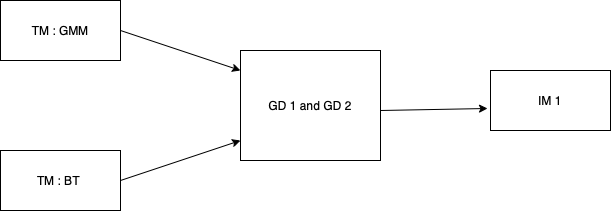
\includegraphics[width=0.6\textwidth]{trace_matrix.png}
\caption{Traceability Graph}
\label{Traceability Graph} 
\end{center}
\end{figure}


% \begin{figure}[h!]
% 	\begin{center}
% 		%\rotatebox{-90}
% 		{
% 			\includegraphics[width=\textwidth]{ATrace.png}
% 		}
% 		\caption{\label{Fig_ATrace} Traceability Matrix Showing the Connections Between Items of Different Sections}
% 	\end{center}
% \end{figure}


% \begin{figure}[h!]
% 	\begin{center}
% 		%\rotatebox{-90}
% 		{
% 			\includegraphics[width=0.7\textwidth]{RTrace.png}
% 		}
% 		\caption{\label{Fig_RTrace} Traceability Matrix Showing the Connections Between Requirements, Instance Models, and Data Constraints}
% 	\end{center}
% \end{figure}

\section{Values of Auxiliary Constants}


\newpage
\nocite{*} 
\bibliographystyle {plainnat}
\bibliography{references} 

\end{document}